\documentclass[a4paper,12pt]{article}  % Basic document class - can use another class if required

% Packages
\usepackage[utf8]{inputenc}             % For UTF-8 encoding
\usepackage[T1]{fontenc}               % For proper font encoding
\usepackage{graphicx}                  % For inserting images
\usepackage{amsmath, amssymb}          % For math symbols
\usepackage{xcolor}                    % For colors
\usepackage{geometry}                  % For page margins
\geometry{margin=1in}                  % Set 1-inch margins
\usepackage{hyperref}                  % For clickable links
\usepackage{biblatex}                  % For bibliography management
\usepackage{algorithm}
\usepackage{algpseudocode}
\usepackage{multicol}
\usepackage{subcaption}                % For subfigures

\addbibresource{report.bib}        % Bibliography file


% Begin the document
\begin{document}

% Title with manually added subtitle
\begin{center}
    \centering  % Center-align the contents
    {\Huge\textbf{Parallel Emperor Penguin Optimizer}\par} % Main Title
    \vspace{0.5cm}
    {\Large High Performance Computing for Data Science Project 2024/2025 \par} % Subtitle
    \vspace{1cm}
    % Two-column layout for authors

    \noindent
    \begin{minipage}[t]{0.5\textwidth} % First Column (45% of the width)
        \centering
        {\large Chiara Marangoni \par}
        {\small mat. 000000 \par} % Add Chiara's ID here
    \end{minipage}%
    \hfill % Add horizontal space between the two minipages
    \begin{minipage}[t]{0.5\textwidth} % Second Column (45% of the width)
        \centering
        {\large Simone De Carli \par}
        {\small mat. 000000 \par} % Add Simone's ID here
    \end{minipage}
    \vspace{1,5cm}
\end{center}  % Include the title page

% Sections of the report
\begin{abstract}
This study presents a parallel implementation of the Emperor Penguin Optimizer (EPO) algorithm, a bio-inspired metaheuristic developed for solving complex optimization problems. 

We enhanced the original EPO algorithm by introducing scaling factors to prevent overshooting and improve solution distribution, then implemented parallelization strategies using both \textbf{MPI} and \textbf{OpenMP} to optimize performance on High-Performance Computing (HPC) clusters. 

The algorithm's effectiveness was validated through comprehensive testing on standard benchmark functions, demonstrating the robustness of our implementation. Performance analysis revealed near-linear speedup with increasing node count and high efficiency, particularly for larger population sizes. 

While the MPI implementation showed promising results, the OpenMP multithreading unexpectedly led to performance degradation, potentially due to memory-related issues.
\end{abstract}



\section{Introduction}

Emperor Penguins Optimization Algorithm (EPO) is a nature-inspired  metaheuristic 
algorithm that takes inspiration from the huddling behavior of emperor penguins, which is a survival strategy to withstand the harsh
Antarctic environment. The algorithm was introduced in 2019 by Dhiman and Kumar \cite{dhiman2018emperor} and has been successfully 
applied to a wide range of optimization problems.

In the context of optimization, metaheuristic algorithms are a class of optimization algorithms that are inspired by natural processes and phenomena. 
These algorithms are typically used to find approximate solutions to complex optimization problems where traditional methods may be inefficient or infeasible. 
Metaheuristic algorithms do not guarantee an optimal solution but aim to find a good enough solution within a reasonable amount of time. 
Examples of metaheuristic algorithms include \textit{Genetic Algorithms} (GA), \textit{Particle Swarm Optimization} (PSO), \textit{Ant Colony Optimization} (ACO), and \textit{Simulated Annealing} (SA).
These algorithms are characterized by their ability to explore and exploit the search space effectively, often using mechanisms such as selection, mutation, crossover, and local search to iteratively improve candidate solutions.
In general population-based algorithms, parallelization can accelerate convergence, enhance exploration, and reduce the likelihood of getting trapped in local optima.\\
This project aims to design and implement parallelization strategies for the Emperor Penguin Optimization Algorithm using and evaluating performance gains achieved through parallelization in terms of speedup, efficiency and scalability.


\section{Related Work}

There is no evidence of the implementation of parallelization strategies for the EPO algorithm, although the problem of parallelization in the field of metaheuristics has been addressed throughout the years \cite{article}.
These strategies generally focus on parallelizing different aspects of metaheuristic algorithms, including solution evaluation, population management, and search processes.   
Parallelization strategies for metaheuristics can be broadly categorized into four main approaches: master-slave, island, cellular models, and hierarchical models. Each of these strategies aims to improve computational efficiency, scalability, and solution quality by distributing workload and enhancing search diversity.
\begin{itemize}
\item The \textbf{master-slave model}, also known as the farm model, is a straightforward approach where a central master process distributes computational tasks, such as fitness evaluations, to multiple worker processes.\newline
\item The \textbf{island model} partitions the population into $k$ smaller subpopulations, or islands, each evolving independently with periodic exchanges of solutions after a defined number of generations $G$.  This approach enhances diversity and prevents premature convergence by allowing different evolutionary processes to explore various regions of the search space before sharing information.\newline
\item The \textbf{cellular model} organizes solutions in a structured spatial layout, typically a $ d $-dimensional grid, where interactions occur locally. \newline
\item The \textbf{hierarchical model} combines multiple levels of parallelism, such as using an island model at a high level while employing master-slave or cellular models within each island. 
\end{itemize}
Beyond these primary models, hybrid and more complex parallelization strategies have been developed \cite{GONG2015286}, integrating elements from multiple approaches and incorporating adaptive mechanisms to optimize performance across different problem domains. 

\section{Methodology}

\subsection{Overview of the Emperor Penguin Optimizer Algorithm}

\begin{algorithm}[H]
    \caption{Emperor Penguin Optimizer (EPO)}
    \label{alg:epo}
    \begin{algorithmic}[1]
    \Require Objective function $f(\mathbf{x})$, population size $N$, maximum iterations $Max_{\text{iter}}$, huddle radius $R$, movement parameters $M$, exploration parameters $f$, exploitation parameters $l$
    
    \State Initialize population of penguins $\vec{P_i}$ $(i = 1, 2, \dots, N)$ randomly

    \State $\vec{P_{\text{best}}} \gets \underset{i}{\arg\min} f(\vec{P_i})$ \Comment{Initialize the best solution}
    
    \While {$itr < Max_{\text{iter}}$}
        \State $R \gets Rand(0, 1)$ \Comment{Random number in the range $[0, 1]$}
        
        \If {$R > 1$}
            \State $T \gets 0$
        \Else
            \State $T \gets 1$
        \EndIf

        \State $T' \gets (T - \frac{Max_{\text{iter}}}{itr - Max_{\text{iter}}})$ \Comment{Compute the temperature profile}

        \State $S \gets \Bigl(\sqrt{f\cdot\exp^{-itr/l}-\exp{-itr}}\Bigr)^2$ \Comment{Compute the social force}

        \For {$i = 1$ to $N$}
            \State $\vec{C} \gets Rand(0, 1)$ \Comment{Generate the avoidance vector}
            
            \State $\vec{A} \gets (M \cdot (T' + |\vec{P_{\text{best}}} - \vec{P_i}|)) \cdot R - T'$ \Comment{Compute the movement vector}

            \State $\vec{D} \gets |S \cdot \vec{P_i} - \vec{C} \cdot \vec{P_{\text{best}}}|$ \Comment{Compute the distance vector}

            \State $\vec{P_i} \gets \vec{P_{\text{best}}} - \vec{A} \cdot \vec{D}$ \Comment{Update the position of the penguin}
            \State Clamp $\vec{P_i}$ to the search space bounds
        \EndFor

        \If {$\underset{i}{\min} f(\vec{P_i}) < f(\vec{P_{\text{best}}})$} \Comment{If a better solution is found}

            \State $\vec{P_{\text{best}}} \gets \underset{i}{\arg\min} f(\vec{P_i})$ \Comment{Update the best solution}
        \EndIf

        \State $i \gets i + 1$
    \EndWhile
  
    \State \Return $\vec{P_{\text{best}}}$

    \end{algorithmic}
\end{algorithm}

\subsection{Our Implementation}


\subsection{Parallelization Strategies}



\section{Experimental Setup}

To evaluate the performance of the proposed algorithm, we conducted experiments on the High-Performance Computing (HPC) cluster at the University of Trento, which operates on the Altaris PBS Professional cluster management software.  
This section provides a detailed description of the computational resources allocated, software environment and evaluation metrics. 


\subsection{Computational Resources}  
The following PBS resource request was used for our experiments:  
\begin{multicols}{2}
\begin{itemize}  
    \item \textbf{Nodes:} 5  
    \item \textbf{CPUs per Node:} 10  
    \item \textbf{Memory per Node:} 2 GB  
    \item \textbf{Operating System:} CentOS 7  
\end{itemize}  
\end{multicols}

\subsection{Software and Compiler Configuration}
To ensure efficient execution of the optimization algorithm, the following software and compiler configurations were used:
\begin{multicols}{2}
\begin{itemize}
    \item \textbf{Programming Language:}  C
    \item \textbf{Parallel Computing Frameworks:} \\ MPICH 4.1.1, OpenMP 3.1
    \item \textbf{Compiler:} \\ GCC 4.8.5 with \texttt{-fopenmp} for OpenMP support
    \item \textbf{MPI Compilation:} \\ \texttt{mpicc} (MPICH) with standard MPI flags
    \item \textbf{Additional Libraries:} \\ Standard C math library (\texttt{libm})
\end{itemize}  
\end{multicols}


\subsection{Evaluation Metrics}
To assess the performance of the algorithm, we considered the following metrics:

\subsubsection{Solution Accuracy}
The accuracy of the obtained solution is measured as the difference between the final solution \( x_{\text{final}} \) and the global optimum \( x^* \):
\begin{equation}
    E = | f(x_{\text{final}}) - f(x^*) |
\end{equation}

\subsubsection{Speedup}
Speedup measures the performance improvement gained by using a parallel program compared to a serial program. It is defined as:
\begin{equation}
    S(P) = \frac{T(1)}{T(P)}
\end{equation}
where:
\begin{itemize}
    \item \( T(1) \) is the execution time of the serial program.
    \item \( T(P) \) is the execution time of the parallel program using \(P\) nodes.
\end{itemize}
In an ideal case, the speedup should be linear, meaning \( S(P) = P \), but due to communication overhead and synchronization, it is often sublinear.

\subsubsection{Efficiency}
Efficiency measures how well computational resources are utilized in a parallel system. It is defined as:
\begin{equation}
    E(P) = \frac{S(P)}{P} = \frac{T(1)}{P \cdot T(P)}
\end{equation}
where:
\begin{itemize}
    \item \( S(P) \) is the speedup.
    \item \( P \) is the number of nodes.
\end{itemize}
Efficiency values range between \( 0 \) and \( 1 \), with \( E(P) = 1 \) indicating perfect efficiency.

\subsubsection{Scalability}
Scalability assesses how well the algorithm maintains efficiency when the problem size and number of nodes increase. It can be analyzed using two models:

\paragraph{Strong Scalability}
Strong scalability examines how execution time decreases when the number of cores increases, while keeping the problem size fixed. Ideally, if an algorithm scales perfectly, the execution time should decrease proportionally to \( P \). Strong scalability is defined as:
\begin{equation}
    S_{\text{strong}}(P) = \frac{T(1)}{T(P)}
\end{equation}
where:
\begin{itemize}
    \item \( T(1) \) is the execution time using a single node.
    \item \( T(P) \) is the execution time using \( P \) nodes for the same problem size.
\end{itemize}
For perfect strong scalability, \( S_{\text{strong}}(P) = P \), but in practice, communication and synchronization overheads reduce the actual speedup.

\paragraph{Weak Scalability}
Weak scalability measures how well an algorithm maintains efficiency when both the number of nodes and problem size increase proportionally. It is defined as:
\begin{equation}
    S_{\text{weak}}(P) = \frac{T(N)}{T(P, N')}
\end{equation}
where:
\begin{itemize}
    \item \( T(N) \) is the execution time for problem size \( N \) using a single node.
    \item \( T(P, N') \) is the execution time using \( P \) cores for problem size \( N' \), where \( N' = P \times N \).
\end{itemize}
An algorithm exhibits perfect weak scalability if \( S_{\text{weak}}(P) = 1 \), meaning the execution time remains constant as both problem size and node count increase proportionally.




\section{Experimental results}
In this section we outline the results obtained by running the simulations in terms of the chosen performance metrics.
\subsection{Algorithm accuracy}
To evaluate the accuracy of the algorithm, we performed five simulations for each of the five fitness functions while maintaining a fixed number of iterations and population size. For the Sphere, McCormick, Matyas, and Michalewicz functions, we used the default optimization parameters \cite{pepo}. In all simulations, the algorithm successfully converged and found the actual optimal value.  
\newline
However, for the Bukin function, due to its complexity and the presence of numerous local minima, we increased the population size to 400 and set the exploration parameter to 3. Despite these adjustments, the algorithm was still unable to consistently converge in all simulations, as it frequently became trapped in one of the many local minima.  
\newline
For consistency, we reported the deviation from the actual optimal value obtained in the different simulations, as shown in Figure~\ref{fig:bukin_deviation}.
\newline
\begin{figure}[h]
    \centering
    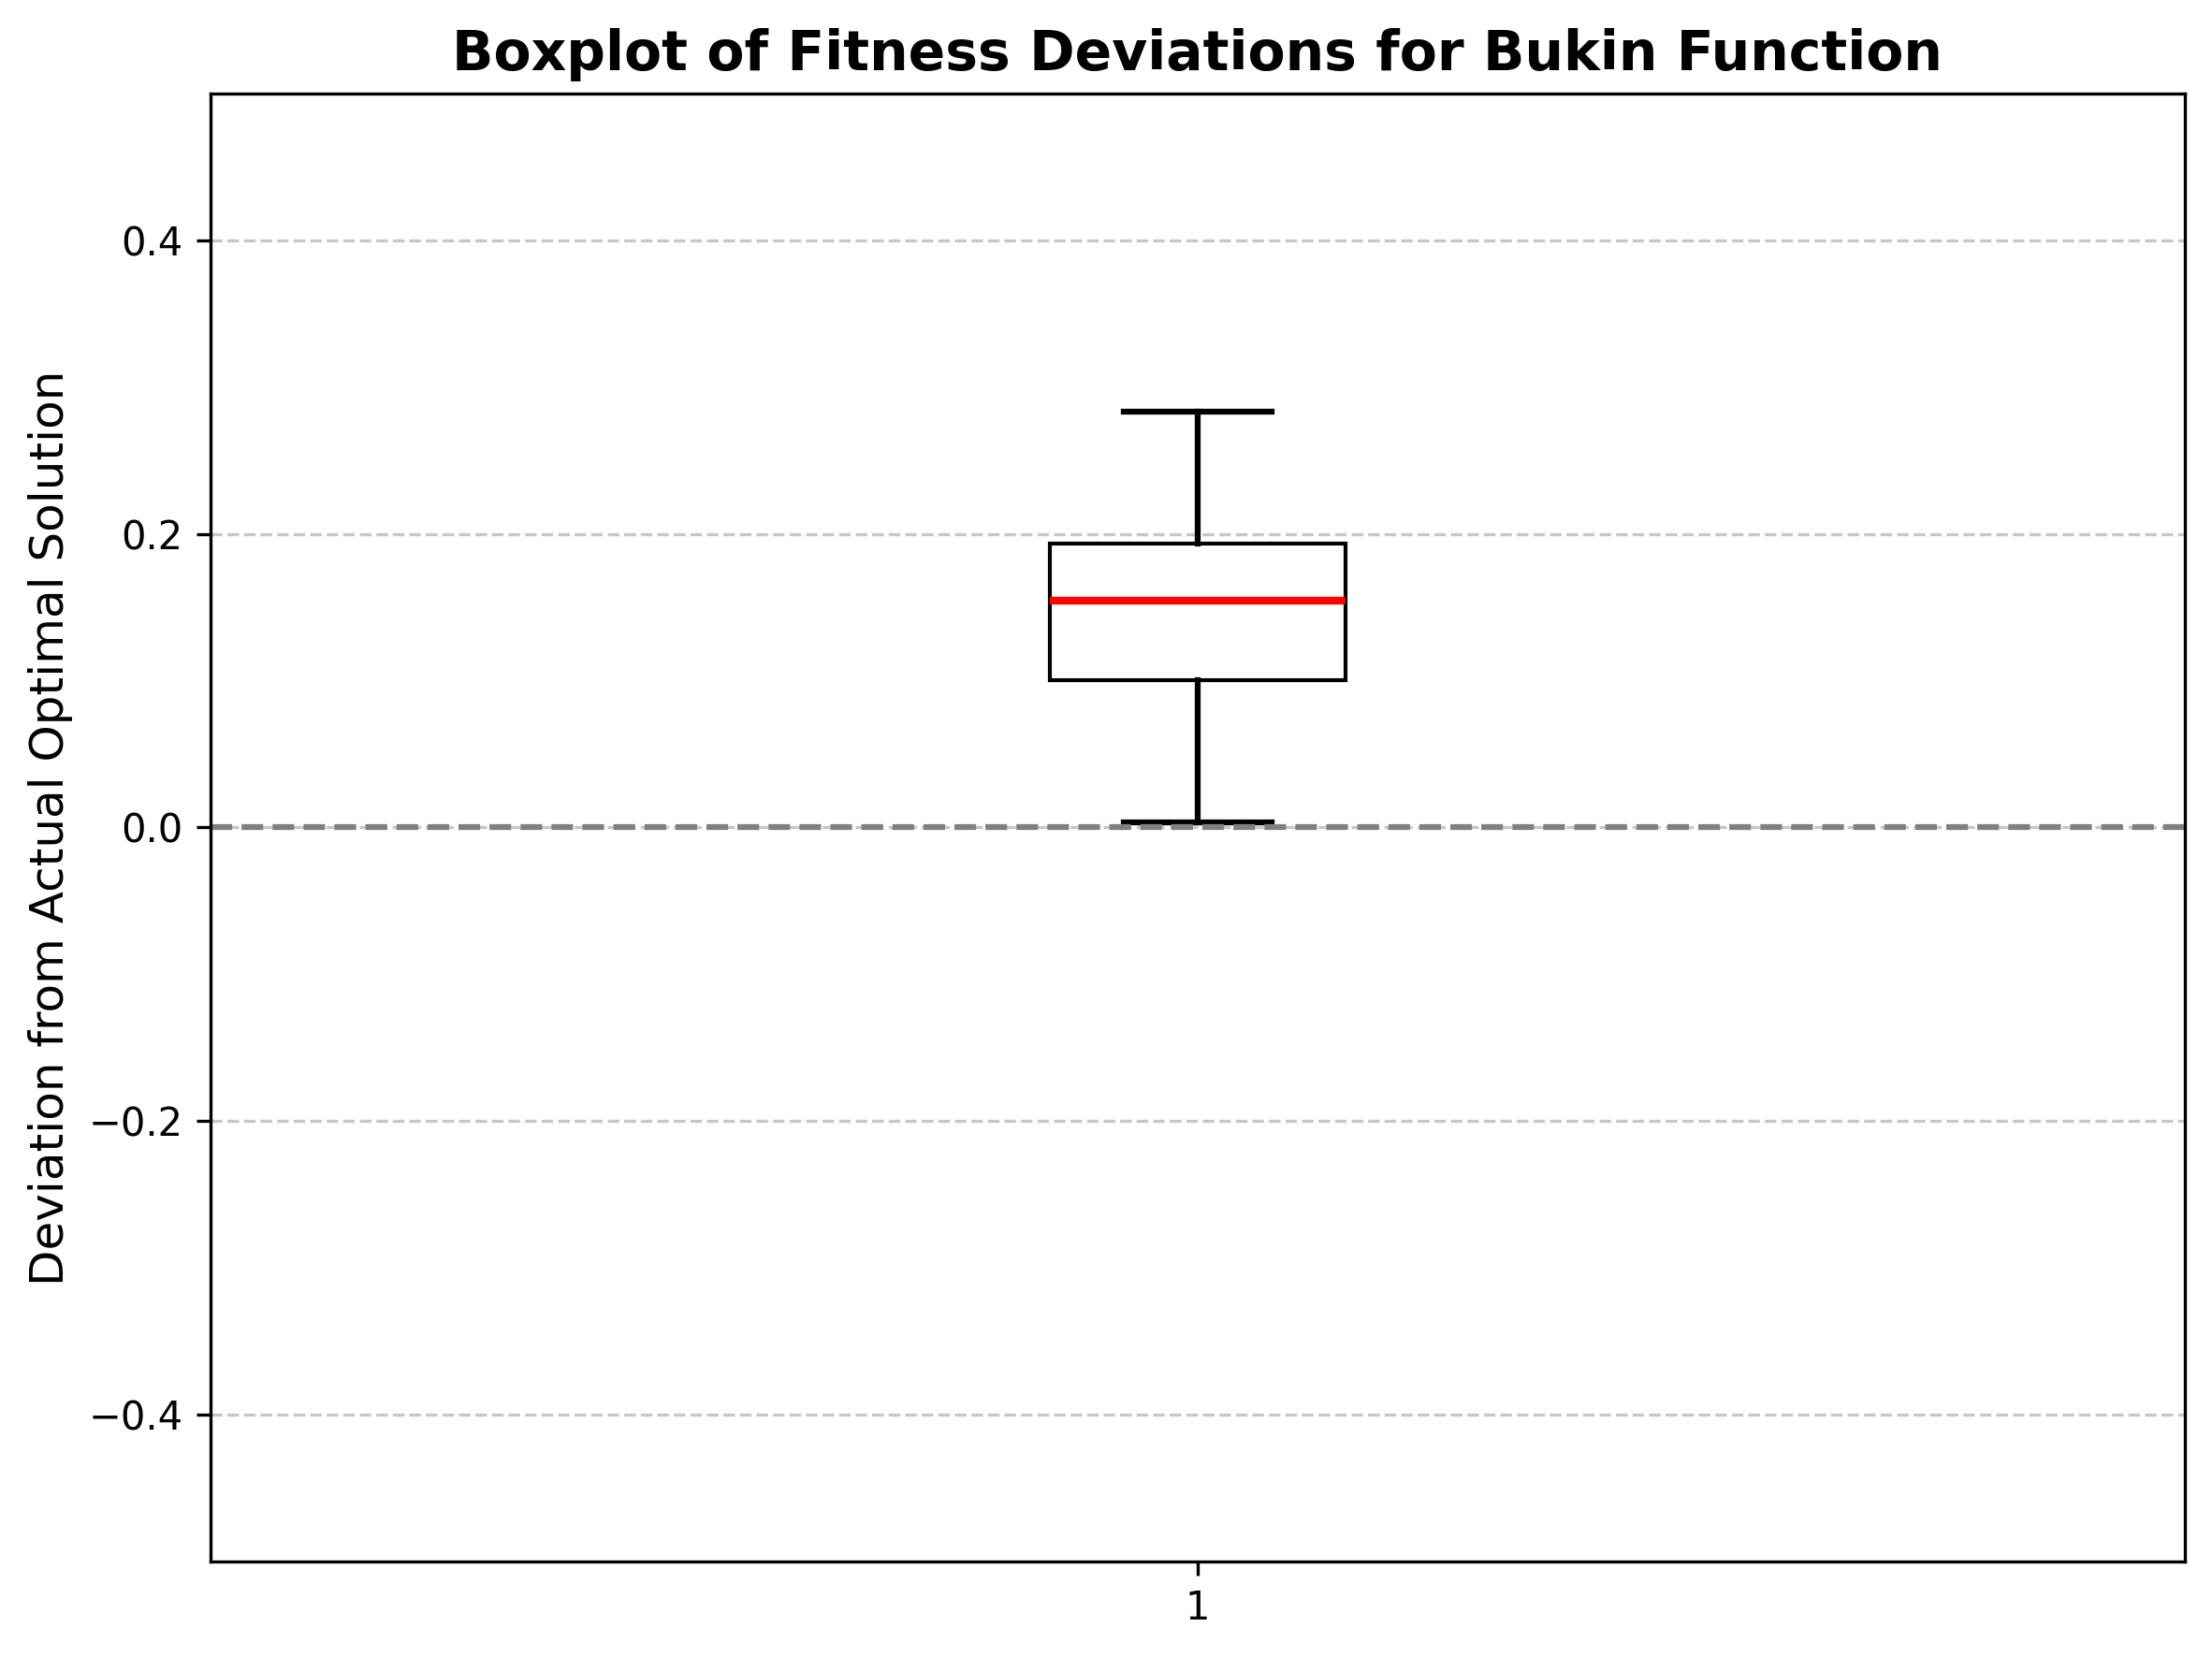
\includegraphics[width=0.5\textwidth]{figures/bukin_fitness_boxplot.png} % Adjust file name if necessary
    \caption{Deviation from the optimal value for the Bukin function.}
    \label{fig:bukin_deviation}
\end{figure}
\newline
\subsection{Parallel performance}
We conducted several simulations of the parallel algorithm, varying the number of nodes and threads from 1 to 50 and the population size. Since our goal was to analyze parallelization performance, we considered the optimization parameters to be irrelevant in this context.  
\newline
For consistency, we kept the number of variables fixed at 100, used the Sphere function, and set a constant number of iterations at 500. We will first outline the results obtained with a varying number of nodes, without considering threads.
\subsubsection{Speedup}
Figure ~\ref{fig:nodes_speedup} illustrates the speedup with different problem sizes while increasing the number of nodes.
\newline
\begin{figure}[h]
    \centering
    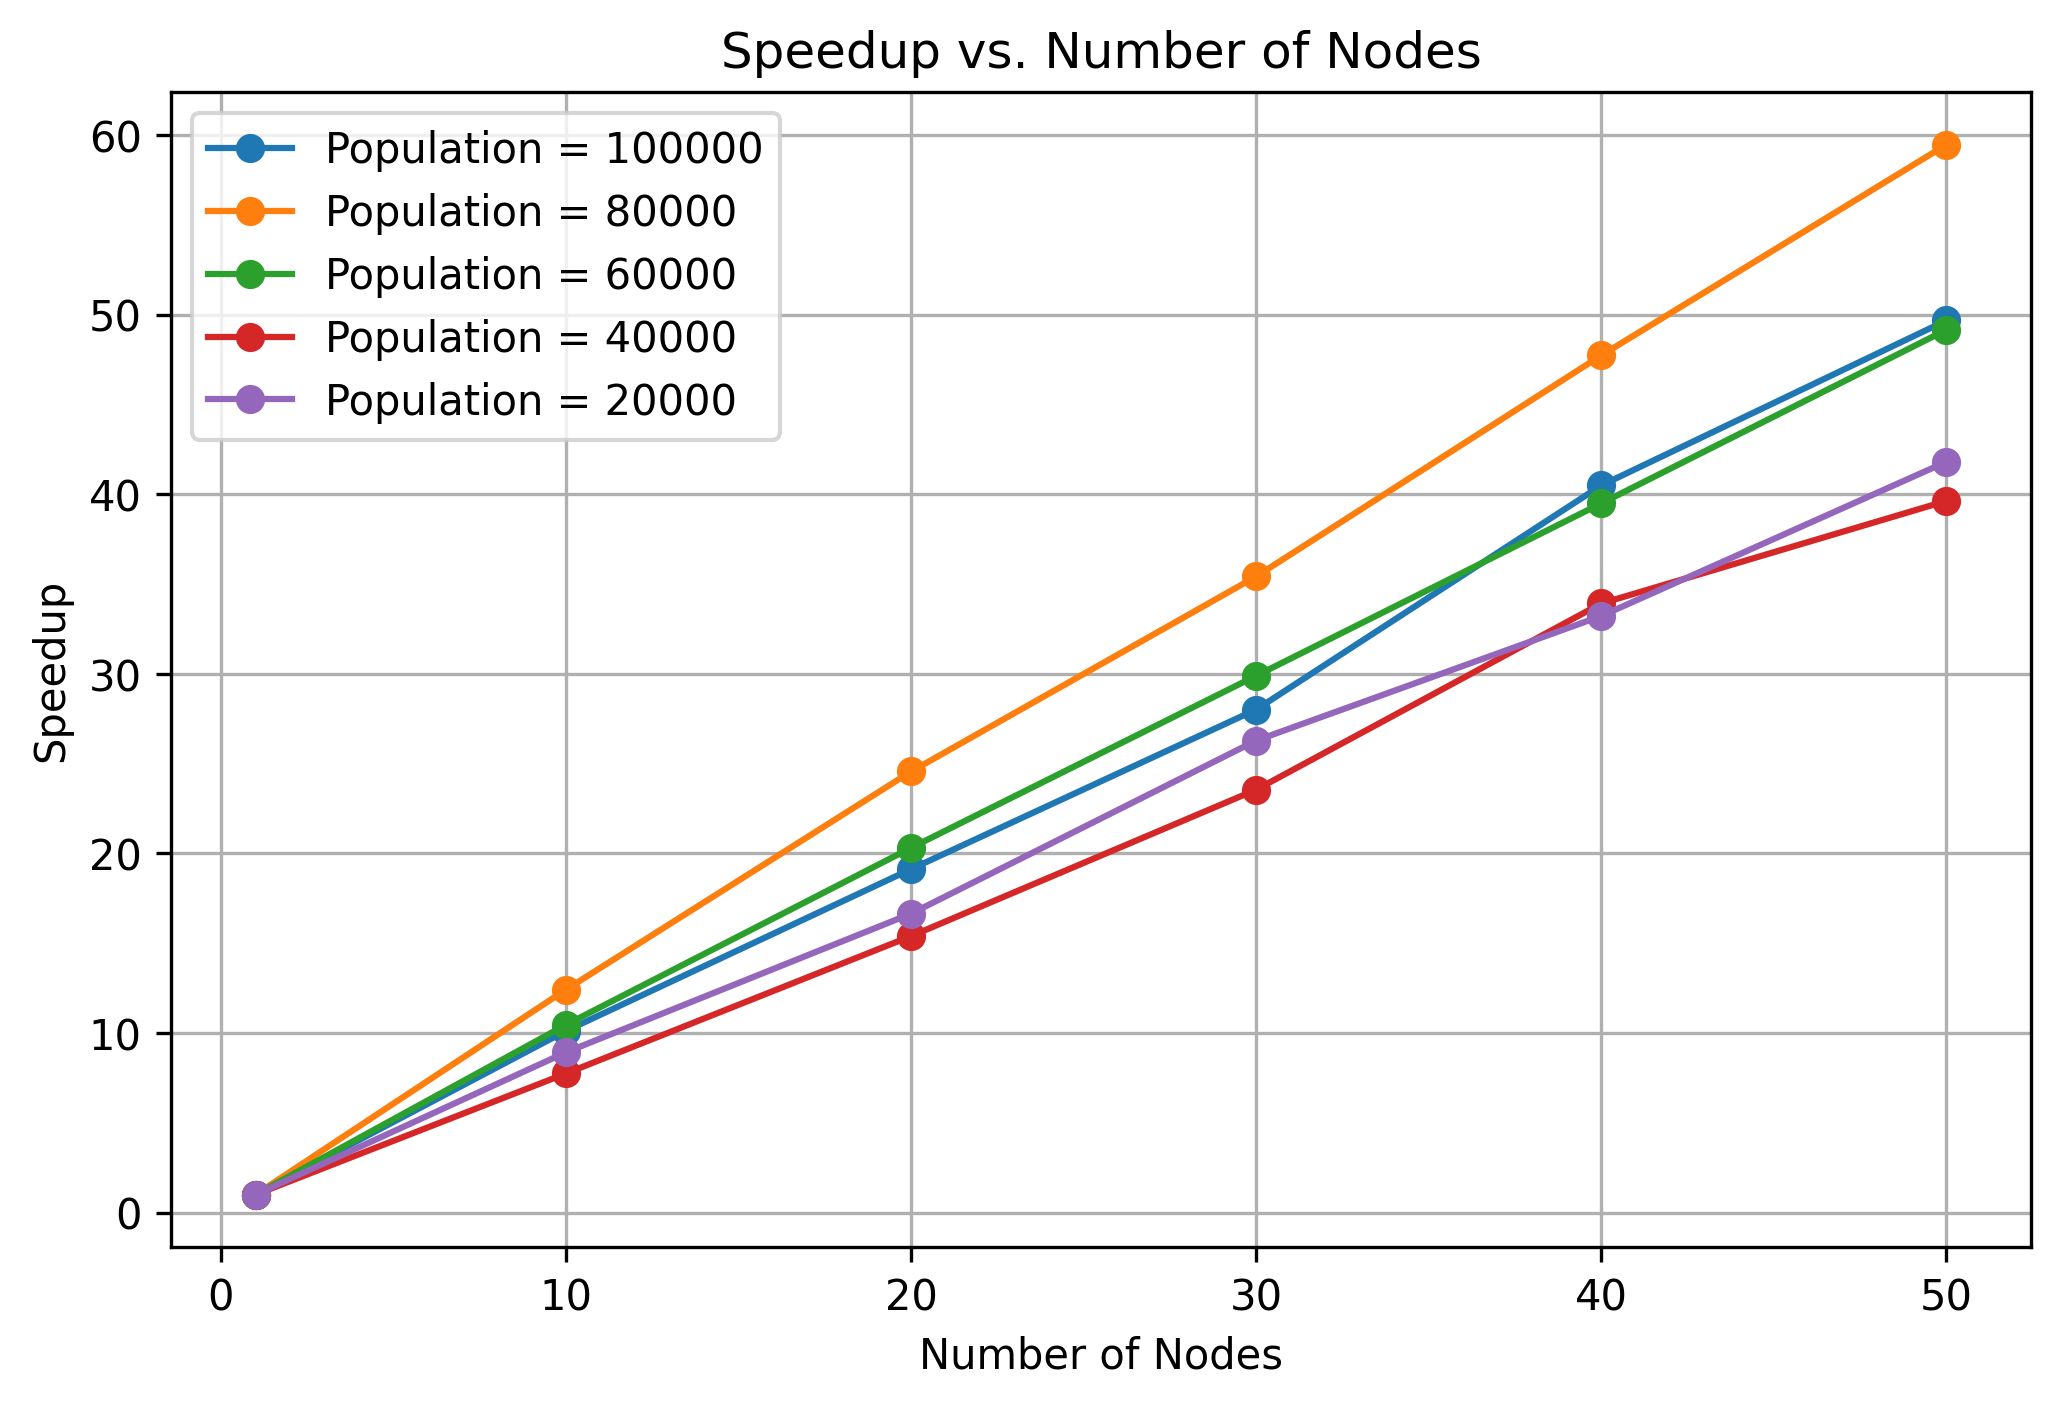
\includegraphics[width=0.5\textwidth]{figures/speedup_vs_nodes.png} % Adjust file name if necessary
    \caption{Speedup graph for different population sizes.}
    \label{fig:nodes_speedup}
\end{figure}
The observed speedup confirms that parallelization effectively reduces the execution time, especially when larger population sizes are used. The speedup increases almost linearly with the number of nodes, which is a strong indicator of good parallel performance.
The different population sizes generally follow a similar trend, though the population of 80,000 shows the highest speedup. This suggests that some problem sizes benefit more from parallelization, potentially due to better workload distribution.
A slight deviation from perfect linear scaling at higher node counts suggests that communication overhead or other bottlenecks might start playing a role.

\subsubsection{Efficiency}
Figure ~\ref{fig:nodes_efficiency} illustrates the efficiency with different problem sizes while increasing the number of nodes.
\newline
\begin{figure}[h]
    \centering
    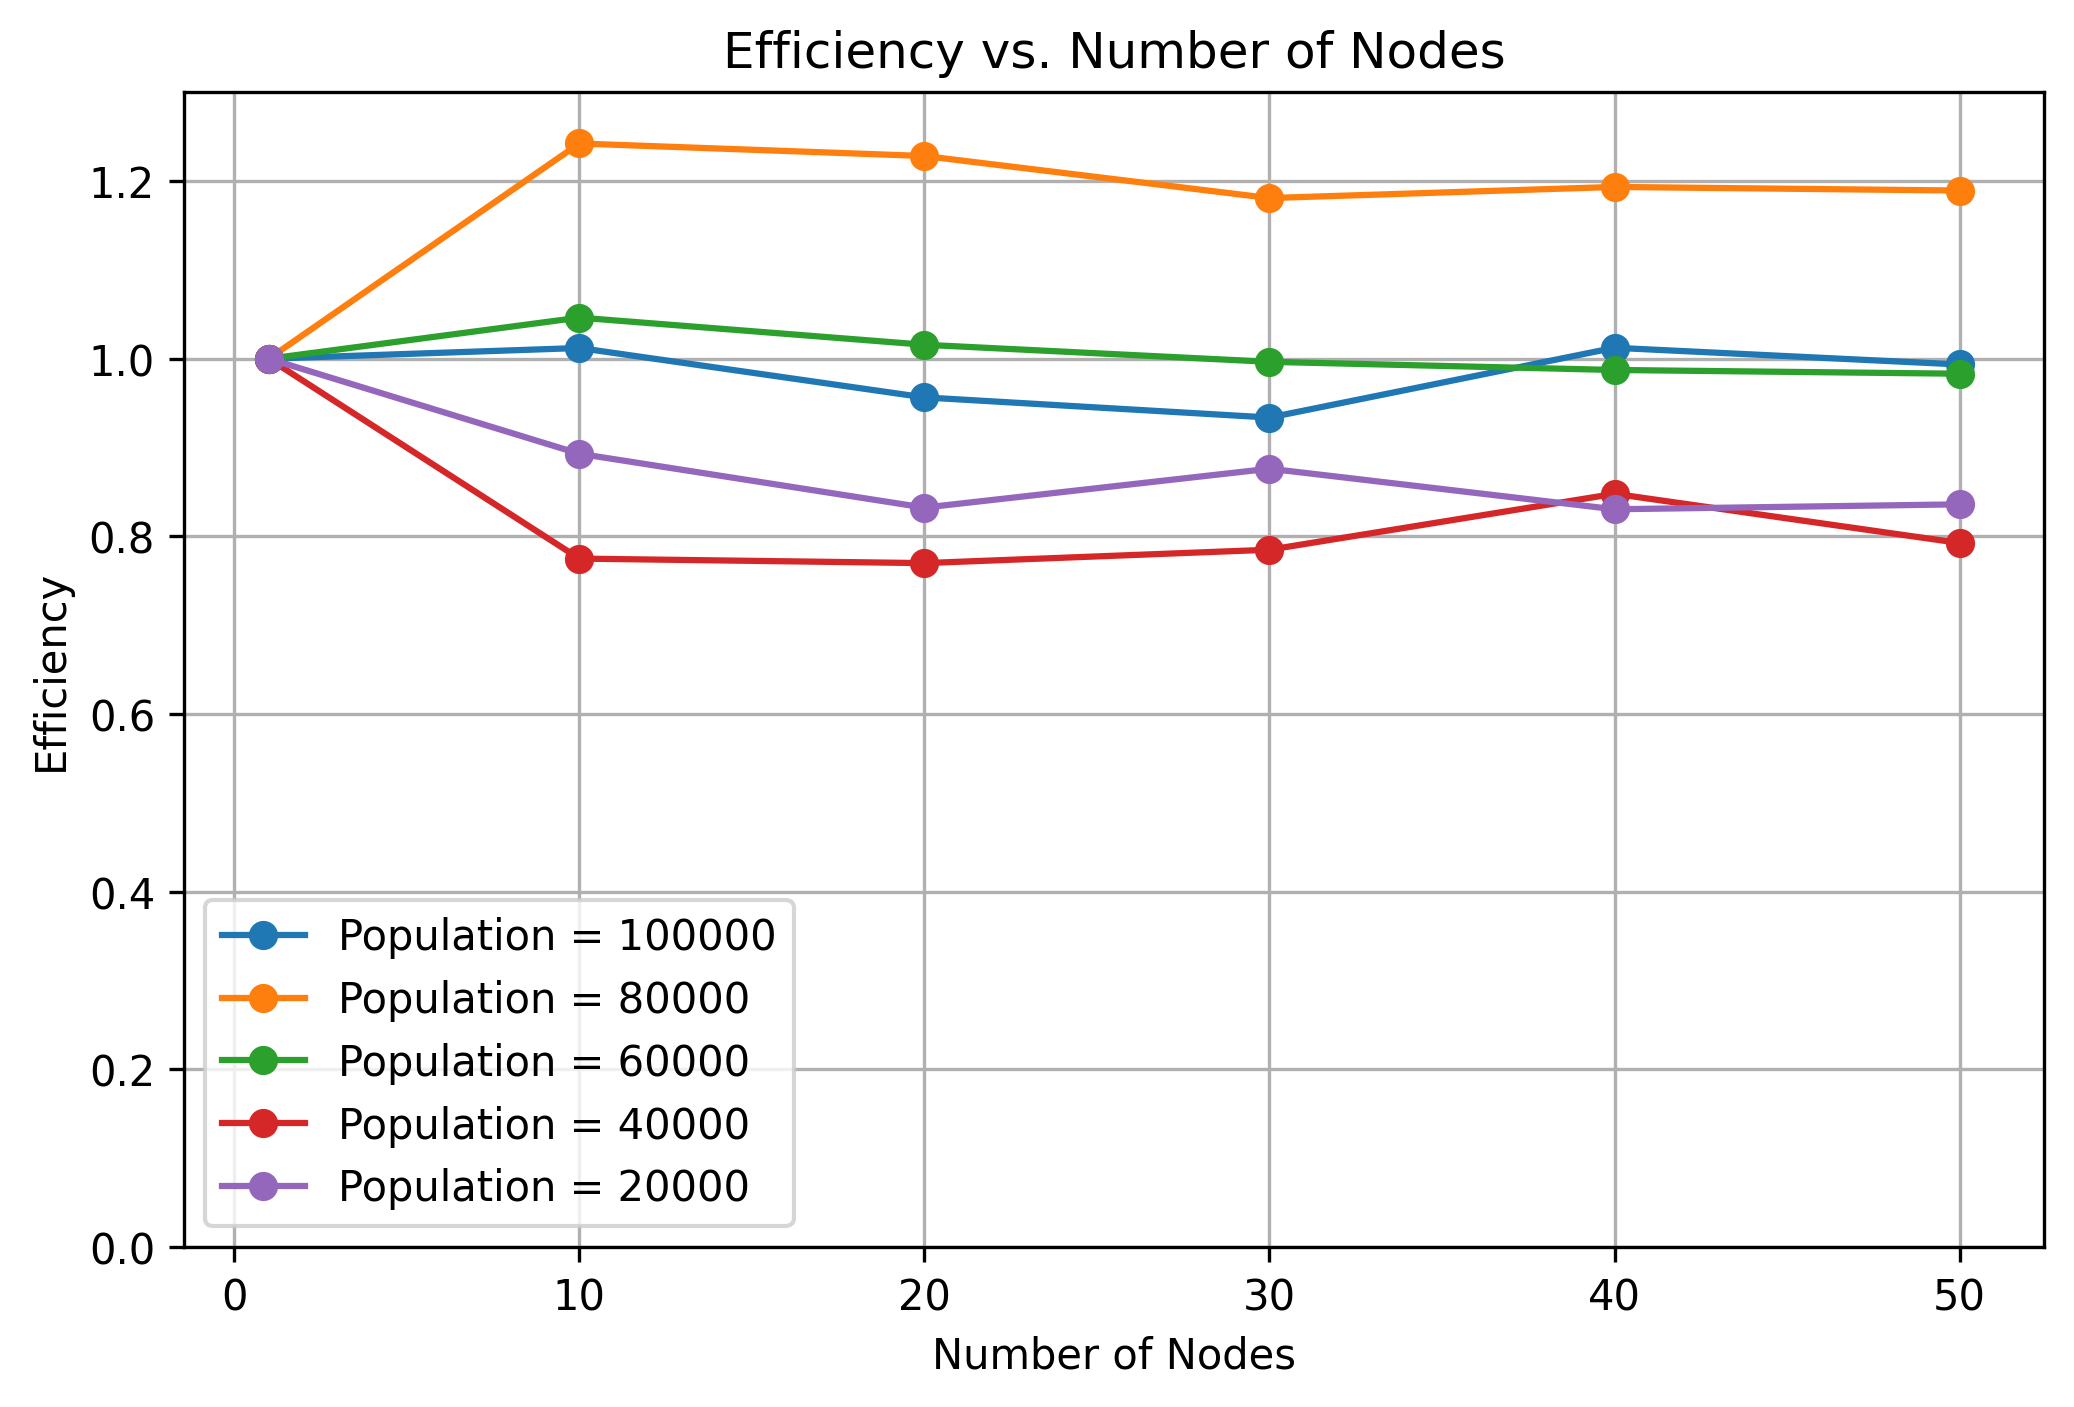
\includegraphics[width=0.5\textwidth]{figures/efficiency_vs_nodes.png} % Adjust file name if necessary
    \caption{Efficiency graph for different population sizes.}
    \label{fig:nodes_efficiency}
\end{figure}
Efficiency mostly remains above or near 1 for larger problem sizes, which is very promising.
The efficiency for the smallest population sizes (20,000 and 40,000) degrades slightly, indicating that these workloads may be too small to benefit from parallelization at higher node counts.
The fact that the efficiency for a population of 80,000 is above 1 suggests a superlinear speedup. While the specific cause of this behavior is not clear, we hypothesize that the heterogeneity of the cluster and the allocation of resources introduce a certain variability, which in turn can affect performance.
\subsubsection{Scalability}
The algorithm demonstrates good strong scaling, as shown in the speedup graph. Figure ~\ref{fig:nodes_scalability} illustrates the weak scalability while increasing the number of nodes.
\begin{figure}[h]
    \centering
    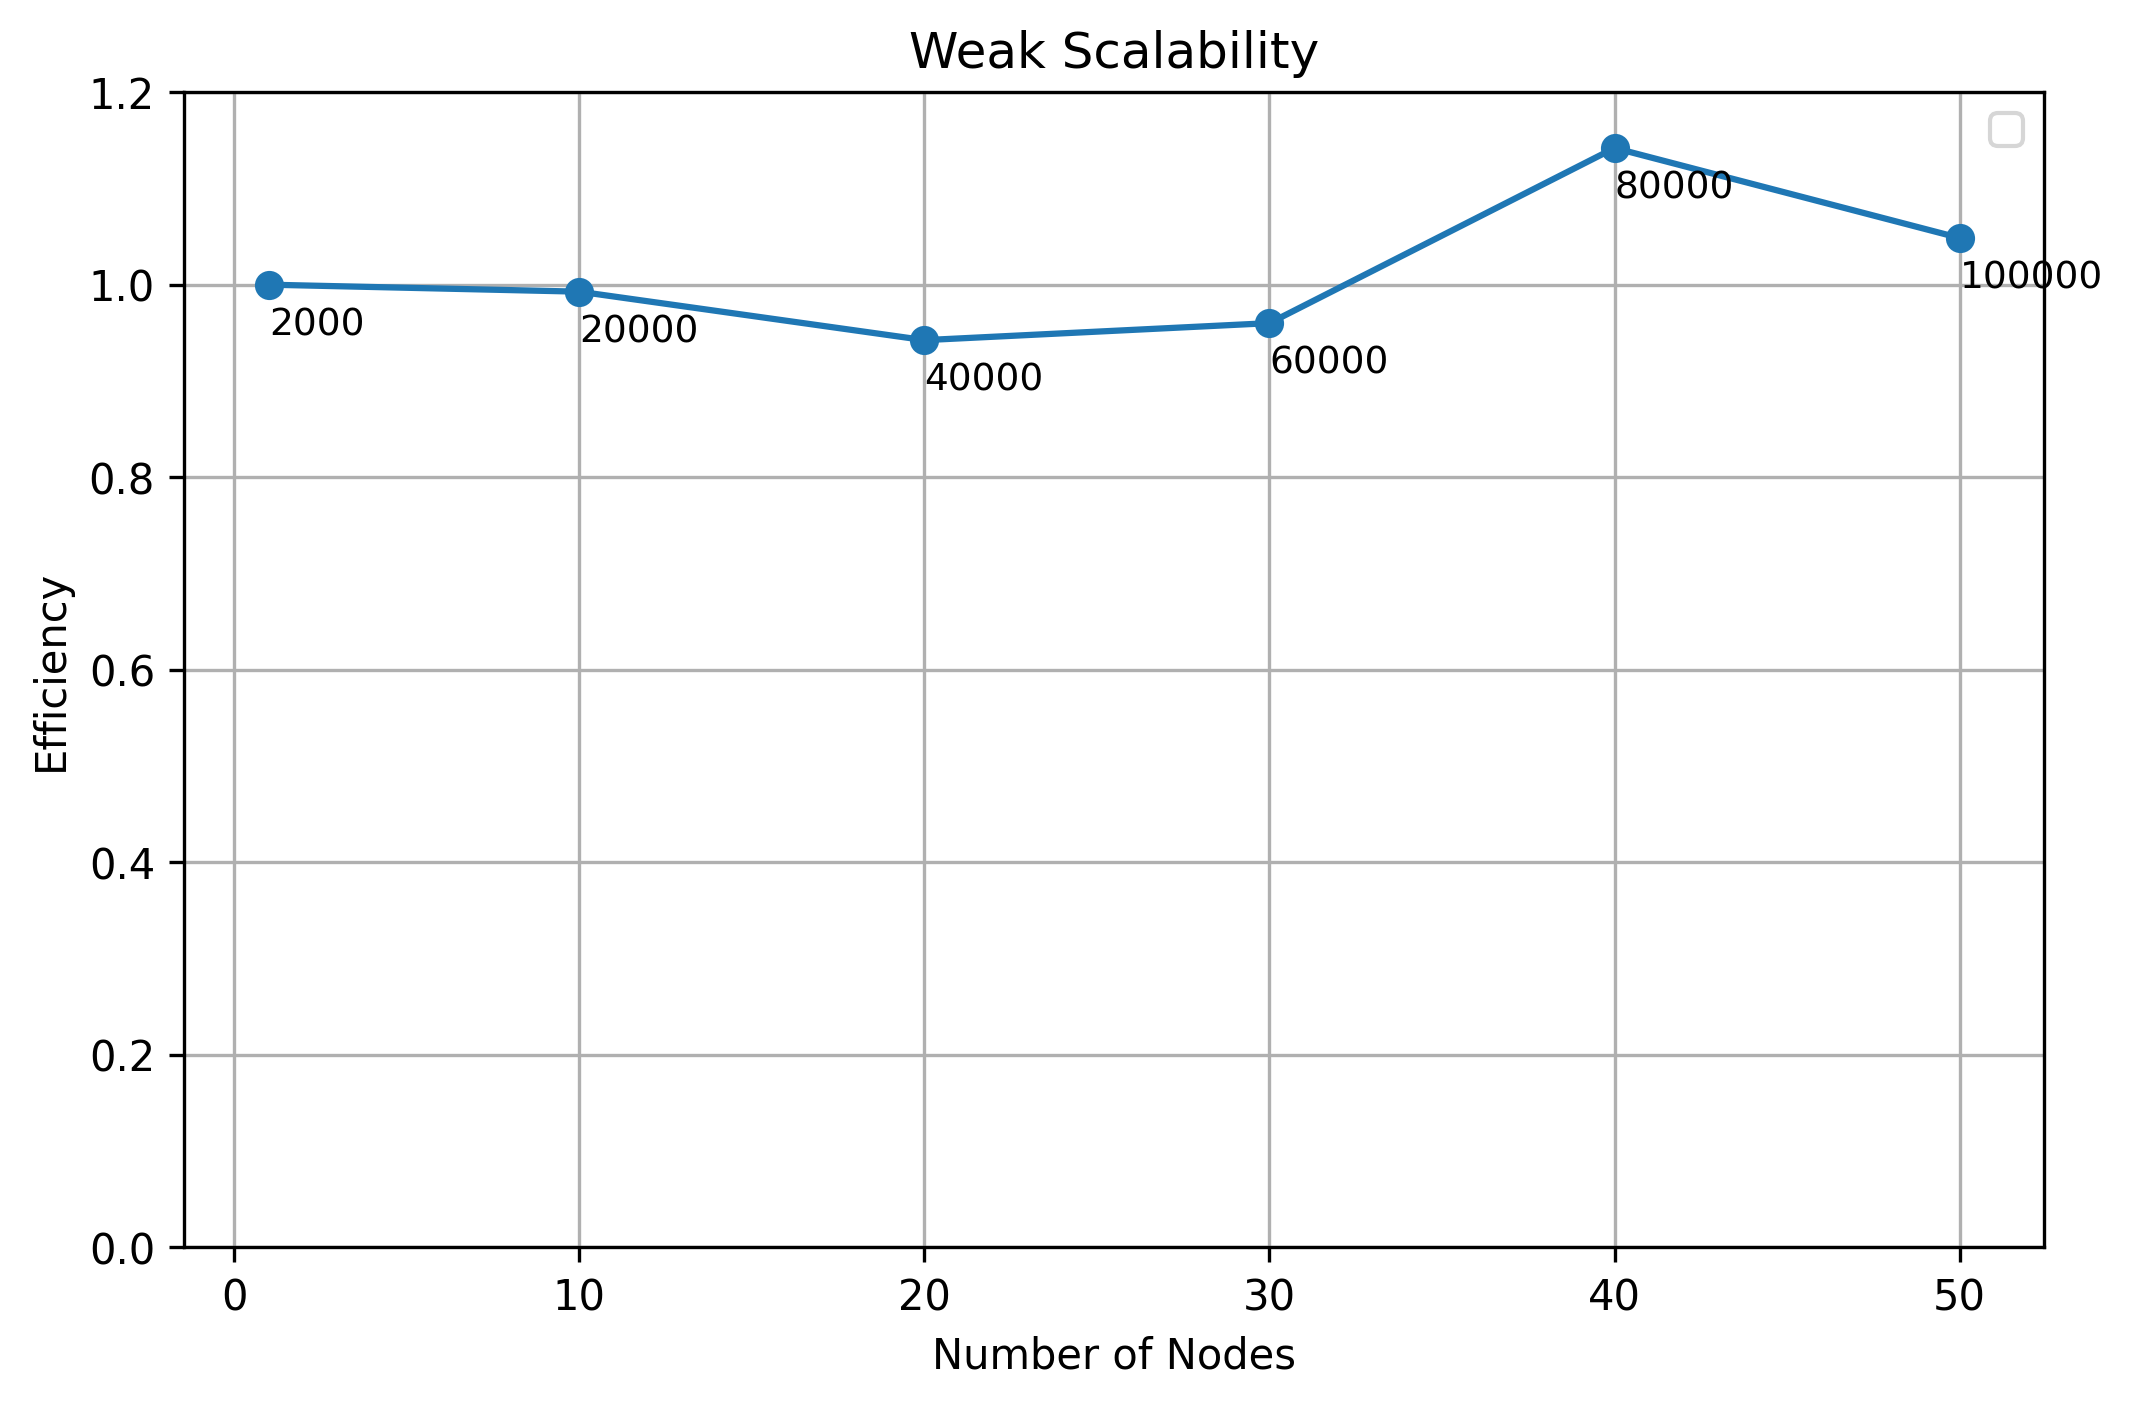
\includegraphics[width=0.5\textwidth]{figures/weak_scalability.png} % Adjust file name if necessary
    \caption{Weak scalability with population size varying from 2000 to 100000}
    \label{fig:nodes_scalability}
\end{figure}
\newline
The efficiency remains around 1 for most cases, which indicates strong weak scaling performance.
A small dip in efficiency around mid-range problem sizes (40,000 and 60,000) suggests potential inefficiencies, but it recovers for the larger problem sizes.
Overall, this result is promising because it indicates that as the problem size grows proportionally with the number of nodes, efficiency remains stable.
\newline
\newline
We conducted the same experiments as with nodes, but using threads to leverage multithreading. However, we observed a degradation in performance. This suggests that our algorithm scales better with distributed computing than with shared-memory parallelism.
\begin{figure}[h]
    \centering
    \begin{subfigure}{0.45\textwidth}
        \centering
        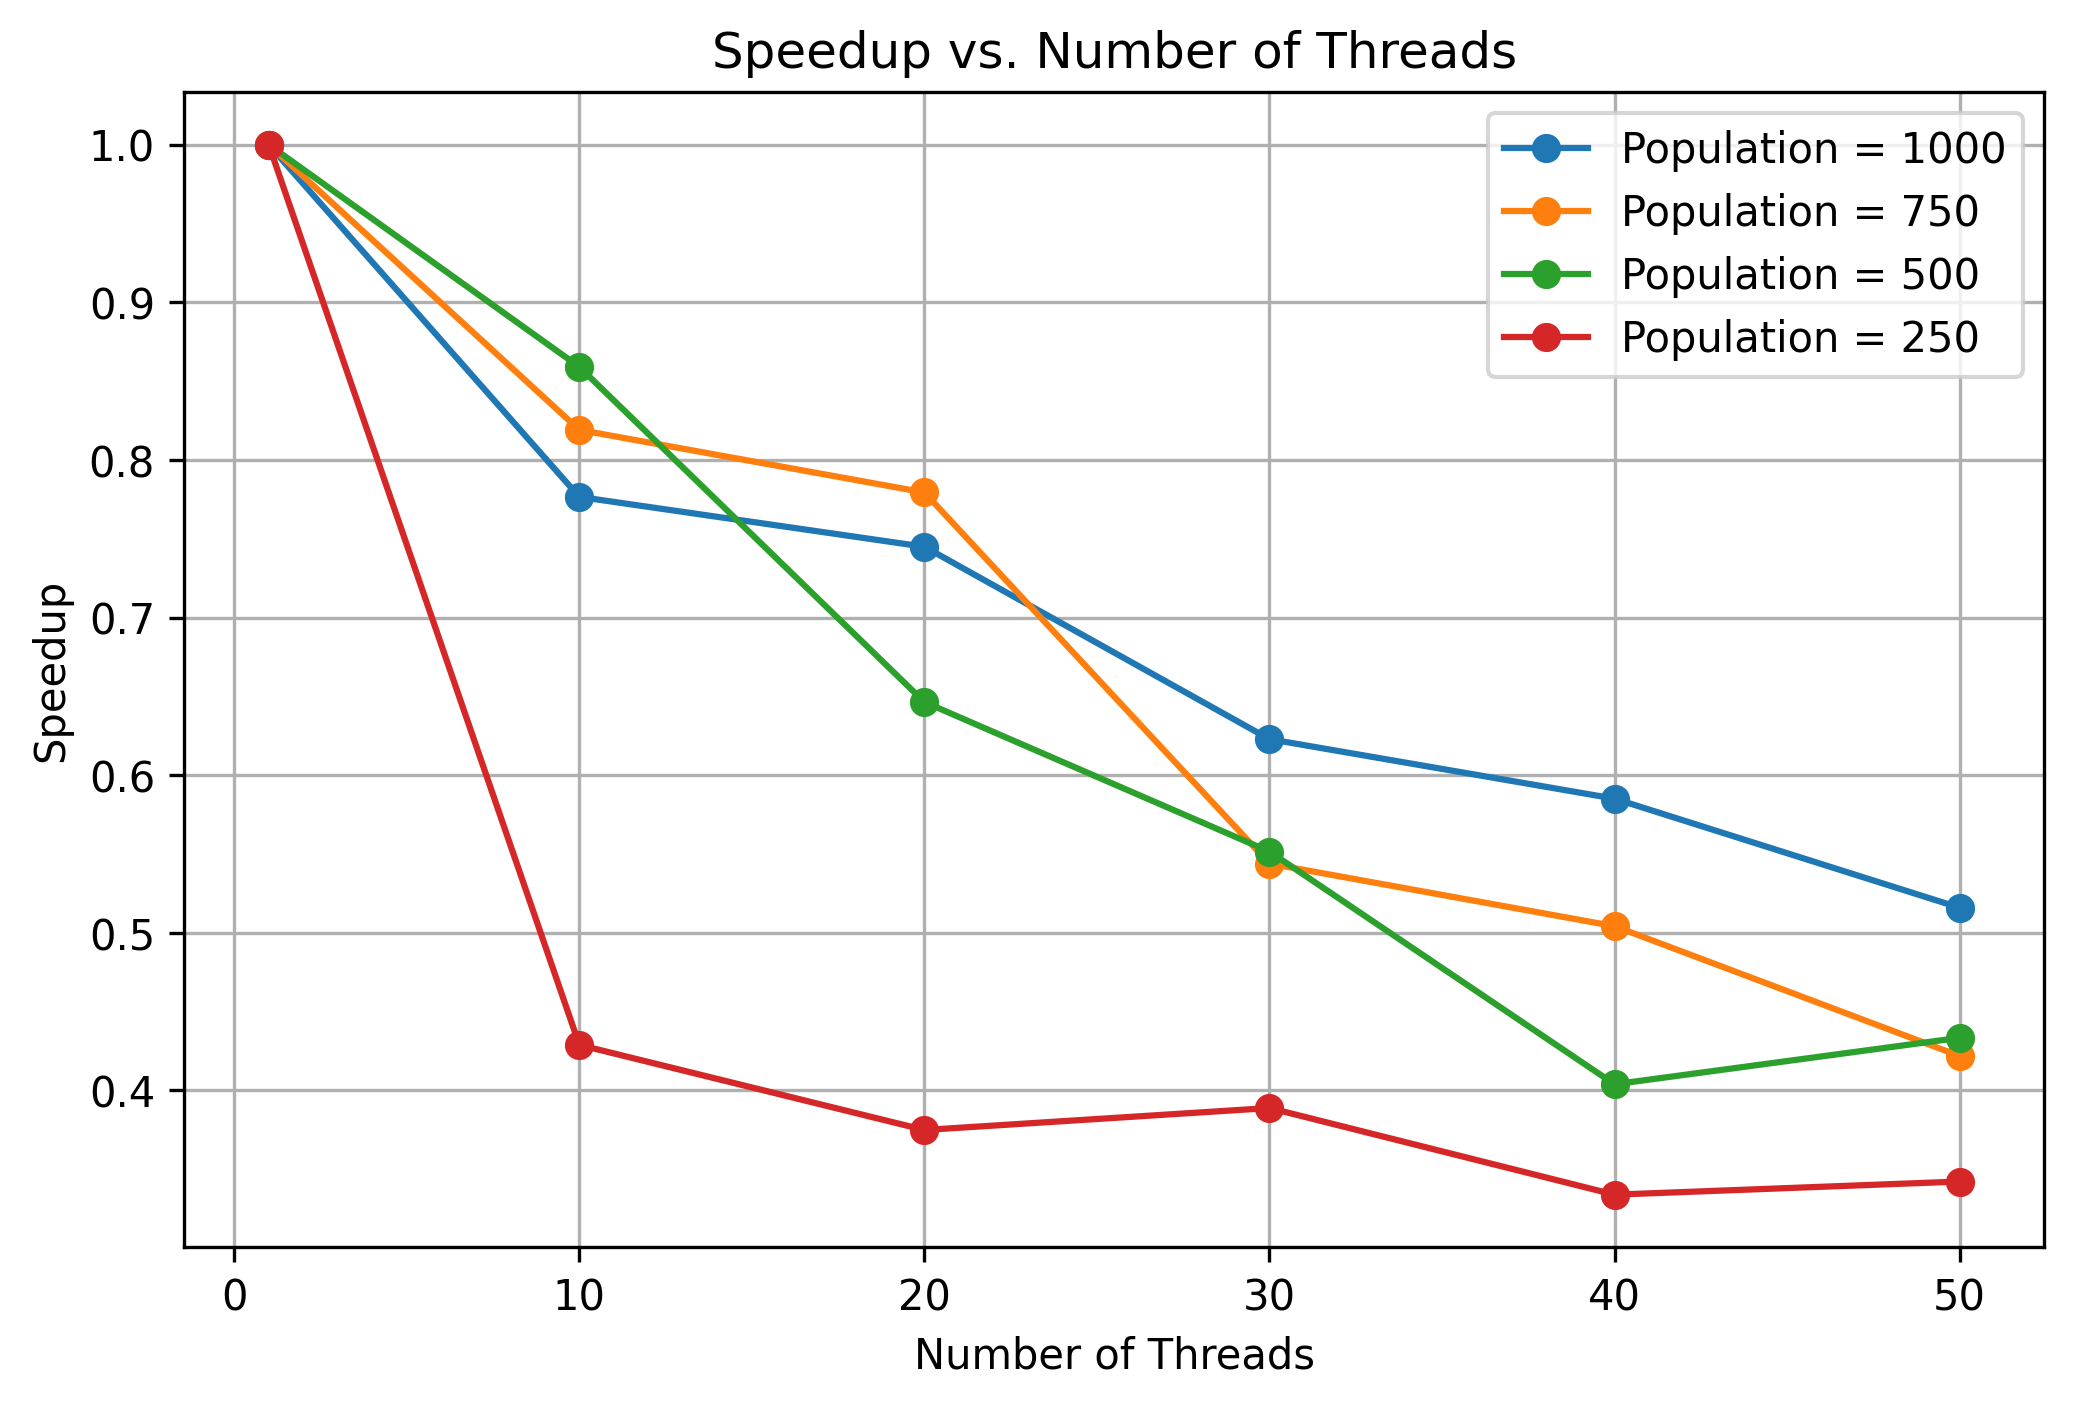
\includegraphics[width=\linewidth]{figures/speedup_vs_threads.png}
        \caption{Speedup vs. Number of Threads}
    \end{subfigure}
    \hfill
    \begin{subfigure}{0.45\textwidth}
        \centering
        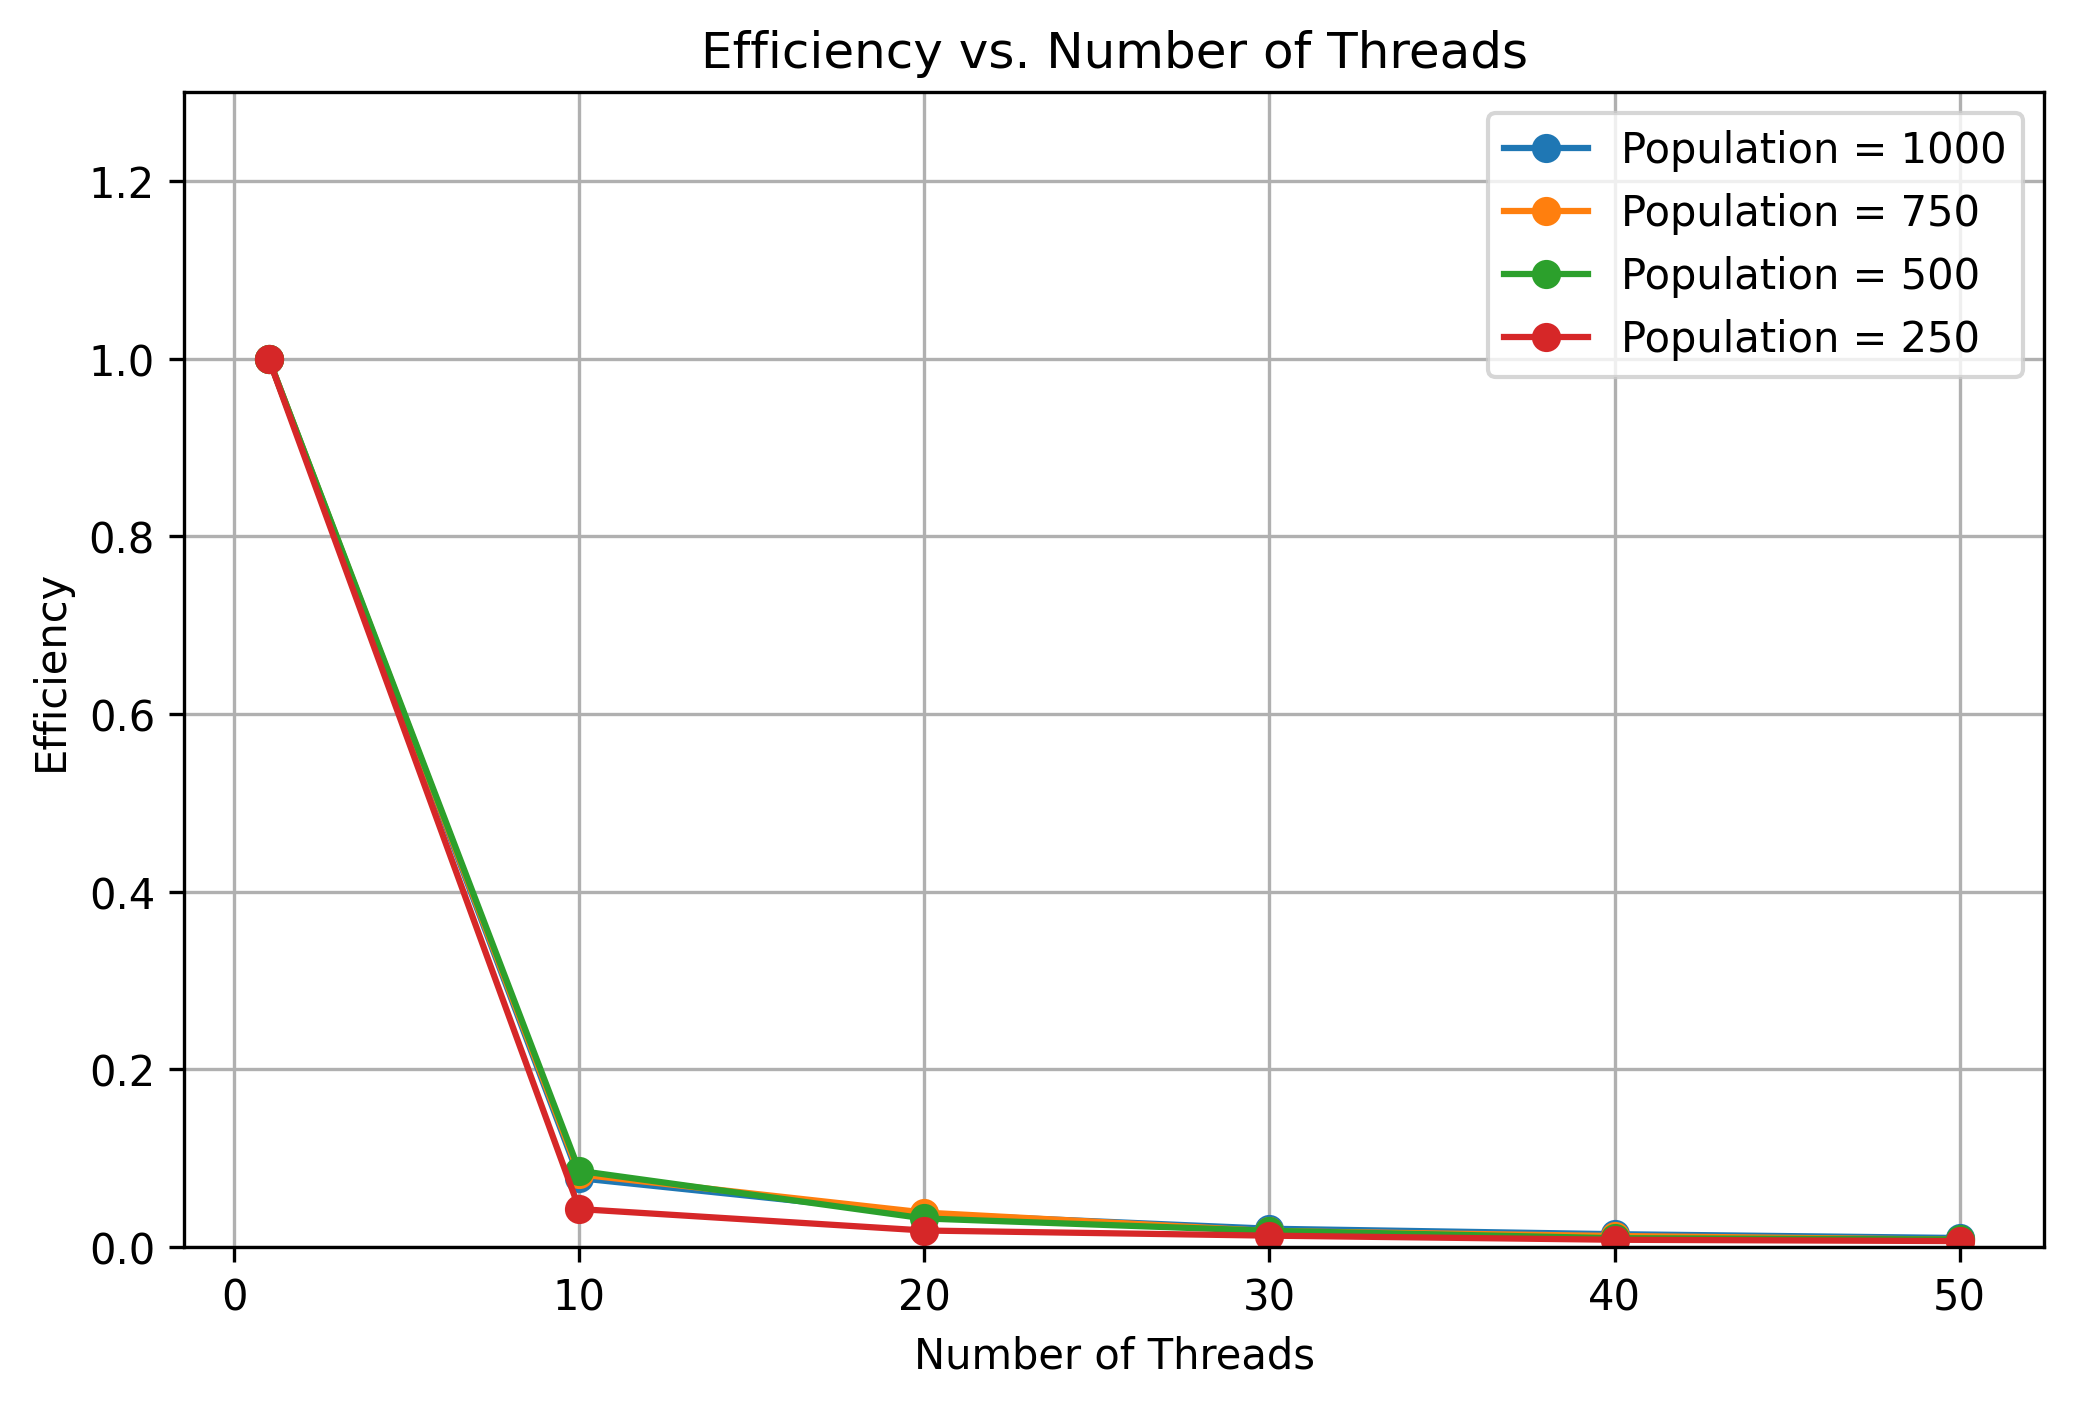
\includegraphics[width=\linewidth]{figures/efficiency_vs_threads.png}
        \caption{Efficiency vs. Number of Threads}
    \end{subfigure}
    \caption{Performance analysis using increasing number of threads.}
    \label{fig:nodes_performance}
\end{figure}
\newline
\subsection{Multithreaded Performance Degradation}
Despite our expectation that multithreading would improve performance, the \textbf{OpenMP} implementation resulted in significant degradation compared to the sequential version. Several potential factors may contribute to this behavior:

\begin{itemize}
    \item \textbf{Scheduling Overhead:} We used dynamic scheduling, which generally introduces more overhead than static scheduling when the workload per thread is uniform. However, extensive empirical testing showed that, despite the relatively even distribution of workload, the dynamic scheduling strategy consistently outperformed static scheduling.

    \item \textbf{False Sharing:} If threads update data stored in contiguous memory locations, cache line contention may occur, leading to performance loss. This could be the case for the temporary arrays allocated per thread, potentially causing frequent cache invalidations.

    \item \textbf{Memory Bandwidth Constraints:} Frequent updates to large data structures might be saturating the available memory bandwidth, making the algorithm memory-bound. This effect could be exacerbated by dynamic memory allocation, which may introduce additional overhead due to inefficient memory access patterns.

    \item \textbf{Granularity of Computation:} The computational load per thread may be too small to offset the overhead associated with thread management, leading to inefficient parallel execution.

    \item \textbf{Allocation Overhead:} Although temporary arrays are allocated outside the parallel loop, their allocation strategy or memory alignment might still impact performance, particularly if memory fragmentation occurs.
\end{itemize}

Despite extensive testing and multiple modifications to the parallel implementation, we were unable to definitively determine the exact cause of the performance degradation. Further profiling and targeted optimizations (e.g., adjusting memory allocation strategies, reducing false sharing, and analyzing cache behavior) are necessary to gain deeper insights into the issue.



\section{Conclusion}
In conclusion, our parallelized algorithm has demonstrated strong efficiency in solving various optimization problems, showing a high degree of scalability and significant speedup when using multiprocess parallelization. However, our experiments revealed that multithreading did not yield performance improvements.
\newline
\newline
Some limitations of this study include the relatively small number of simulations used for parallel performance assessment, which introduces variability in the results that could have been mitigated by conducting multiple runs. Additionally, our implementation relies heavily on dynamic memory allocation, which may have negatively impacted performance. Another challenge was the absence of an official, formal, and unambiguous description of the algorithm, leading us to base our implementation on unofficial sources. 
\newline
\\
For future work, we suggest conducting multiple simulations to obtain more precise performance measurements and exploring the use of computationally expensive fitness functions to further evaluate scalability and efficiency.

\printbibliography    % Bibliography is printed here

% End the document
\end{document}